\documentclass[12pt]{article}

\usepackage[english]{babel}
\usepackage[utf8x]{inputenc}
\usepackage{chemfig}
\usepackage[version=3]{mhchem}
\usepackage{listings}
\usepackage{graphicx}
\usepackage{enumitem}
%\usepackage{geometry}
%\newgeometry{margin=2cm}
\usepackage[top=3.5cm, bottom=3.5cm, left=2cm, right=2cm]{geometry}
\renewcommand{\baselinestretch}{1.2} 
\begin{document}

\title{\textbf{Schema.org Injector} \\ \emph{Dokumentation} }
\author{Stefan Haberl, Mathias Meinschad \\ \emph{STI Innsbruck}}
\date{WS 2016/17 \\ 
\includegraphics[width=0.25\textwidth, height=0.25\textwidth]{icon.png}}

\maketitle
\newpage

\tableofcontents
\newpage


% % % % % % % % % % % % %
% PROJECT
% % % % % % % % % % % % %
\section{Project}
\subsection{Overview}
The goal of this project was to develop an extension for the CMS-system \textbf{TYPO3}, which allows the users to inject schema.org annotated JSON-LD files into their webpages.

Each page can be associated individually with one or more JSON-LD files, which then are injected dynamically into the page's \textbf{head tag}.

\subsubsection{Specifications}

	We defined the following points to be important requirements to our extension:
	\begin{itemize}
		\item Allow injection of JSON-LD into a single page / multiple pages
		\item The extension should be easy to install and intuitive usage should be guaranteed
		\item Compatibility to as many TYPO3 versions as possible, since older web projects still use version 6 and newer ones already use version 8
	\end{itemize}


\subsection{JSON-LD}
JSON-LD is a method of encoding Linked Data. It is built up on the most common data format used for asynchronous browser/server communication: \textbf{JSON}. As you can see in the example below, JSON-LD just extends JSON with some key words. We will explain some of these later in this documentation.

\subsubsection{Why JSON-LD?}
\begin{itemize}
	\item easy readable for both, humans and machines
	\item standard libraries for nearly any programming language
	\item manipulating HTML directly is not required, like in other schema mark-up methods (RDFa or microdata)
\end{itemize}

\subsubsection{Example of JSON-LD}
Here you can see a minimal example of JSON-LD:
\begin{lstlisting}
	<script type="application/ld+json">
	{
	  "@context": "http://schema.org/",
	  "@type": "Person",
	  "name": "Albert Einstein"
	}
	</script>
\end{lstlisting}
Those keys with an \textbf{@} in front are JSON-LD specific keywords. 

\emph{@context} describes the context of this JSON snippet. E.g. web crawlers know they've found a JSON-LD snippet with content specified by schema.org. 

\emph{@type} tells the application how to interpret the rest of the data. Furthermore it knows what type of data has to be associated with the specific keys.
	


\subsection{Typo3 CMS}
\subsubsection{TYPO3 is \dots{}}
\begin{itemize}
	\item \dots{} an open source CMS (content management system)
	\item \dots{} developed by Kasper Skårhøj
	\item \dots{} released in 1998
	\item \dots{} using several technologies: PHP, SQL und JavaScript
	\item \dots{} rendering pages specified by TypoScript and Fluid
	\item \dots{} currently updated: V8.5.1 (January 25, 2017)
\end{itemize}


% % % % % % % % % % % % %
% OUR EXTENSION
% % % % % % % % % % % % %
\section{Our Extension and how it works}
\subsection{General}

We have developed our extension with JetBrains PhpStorm, which allows syntax highlighting in a very advanced way. From the developer's view TYPO3 can be seen as a framework containing many pre-defined functions and variables. Therefore the whole TYPO3 directory should be included into the PhpStorm project, for instance to be able to jump to a function's declaration. Once installed the project, local testing is done with XAMPP.

TYPO3 uses extension keys to allow unique identifying each extension. This extension key has to be registered at TER (TYPO3 extension repository). We have done this using the key \textbf{schema\textunderscore injector}.

\subsection{How it works}
\begin{figure}[ht]
	\centering
	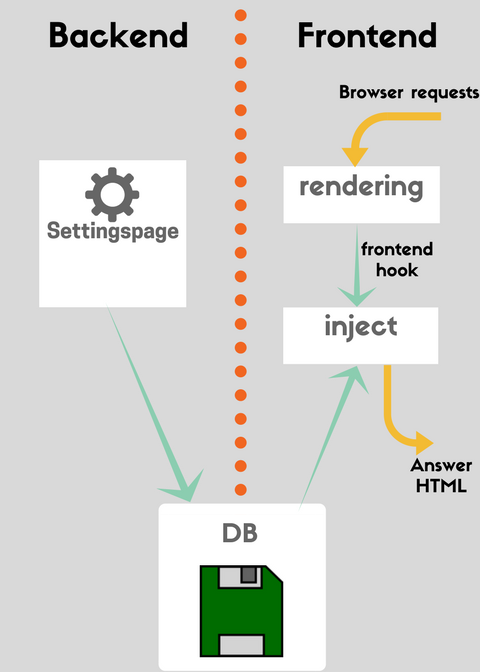
\includegraphics[height=0.75\textwidth]{work_flow.png}
	\caption{This illustration describes how our extension works in Typo3.}
	\label{work_flow}
\end{figure}
As you can see in figure \ref{work_flow} we built a backend module and a frontend plugin (these names are really differentiated by TYPO3).

The backend module displays the user interface and is used to upload JSON-LD files to the server.
Furthermore it is needed to inject uploaded JSON-LD files into pages and also to delete injections from pages.

The frontend plugin includes the below described hooks, which are called each time a page gets rendered. It actually injects the JSON-LD to the rendered page.
Some little file checks are done, e.g. if the schema annotated code snippet already contains script-tags, it leaves them out in the injected code.

\subsection{More technical}

While TYPO3 renders its visible HTML content, there can be defined some functions which are called at a specific point of time in the rendering cycle. 
We are using a frontend hook, which gets called each time a page is rendered.

As you can see in figure \ref{work_flow} the first step is the settings page. When the user adds a page-file association, a row in the database is created, containing the page ID, the file name and an auto-increment universal identifier used as primary key. We have therefore altered the already existing TYPO3 database by a single table called \emph{tx\textunderscore schemainjector\textunderscore domain\textunderscore model\textunderscore injector}. The chosen table name is according to TYPO3 conventions.

The next step is a page request (e.g. HTTP). Nearly at the end of the page's rendering cycle our hook function gets called, which then checks if some entries were made in the database for that specific page ID. If so, the hook injects the content of the JSON-LD file into the raw HTML and continues with returning the manipulated page sources.

% % % % % % % % % % % % %
% Interface
% % % % % % % % % % % % %
\subsection{Interface}
\begin{figure}[ht]
	\centering
	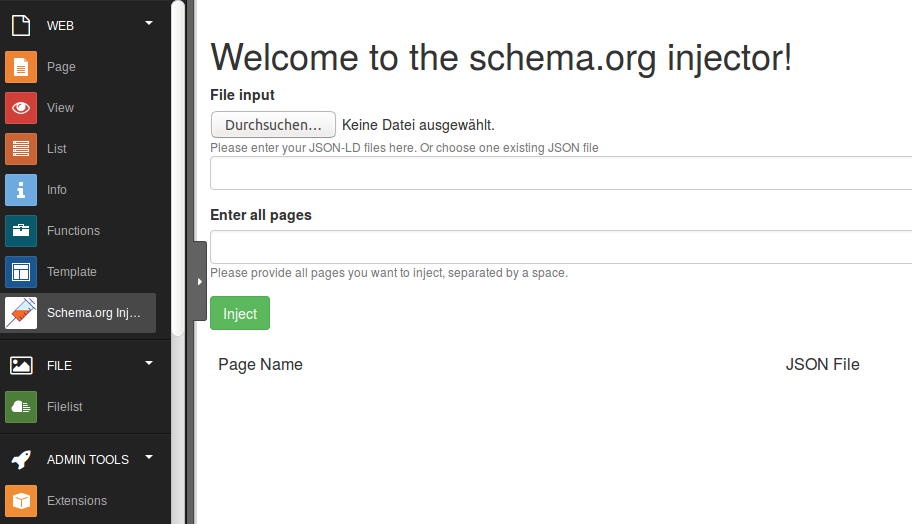
\includegraphics[width=1.0\textwidth]{backend_module.png}
	\caption{This is an image of the interface of our extension.}
	\label{interface}
\end{figure}

As you can see in the figure \ref{interface} our extension is very intuitive and simple to use. On the top of the interface is a file uploader. The user can upload his/her JSON-LD files onto server. We did not make any specific validation tests for those files. It just will be checked if it is a JSON-LD file. The responsibility of a correct JSON-LD file relies on the user.

Below the file uploader it is possible to select an already uploaded JSON-LD file. This field is necessary because having two identically named files is prohibited.

Further down, the page input field is placed. The user has to name all the pages, where the uploaded or selected JSON-LD file should be injected. As a comfort feature the extension allows a wildcard \textbf{\%} and multiple page selection, deliminated by space. For example, inserting the page name \% would select ALL pages.

This section could be easily improved with check boxes of all active pages in TYPO3. Then the user would just have to check all pages where the injection should be done.


% % % % % % % % % % % % %
% OUR PROBLEMS
% % % % % % % % % % % % %
\section{Problems we had}
\begin{itemize}
	\item Initially we had no experience with TYPO3
	\item Caching behaviour in TYPO3 while development (couldn't be completely turned off)
	\item Documentation is often out of date
	\item Small community, nearly no forums
	\item Low basic knowledge in PHP
	\item Solutions for older version not suitable for us
	\item Typo3 in general: TypoScript, how to inject code \dots
\end{itemize}

\section{Conclusion}

At the beginning there were several problems to be solved. Different techniques were tested and looked up. We learned a lot from other extensions which we used for collecting some ideas on how to solve and implement our extension. The work effort was quite suitable for two students because splitting tasks was possible (e.g. frontend/backend, research/testing).

At the end we got an extension which is already published on TER to allow people on the whole globe to inject schema.org annotated files to their webpages. 

\end{document}